\documentclass[12pt, a4paper]{article}
\renewcommand*\contentsname{Inhaltsverzeichnis}
\usepackage[ngerman]{babel}
\usepackage{mathptmx}
\usepackage{blindtext}
\usepackage{subcaption}
\usepackage{emptypage}
\usepackage{wrapfig}
\usepackage[pdftex]{graphicx}
\usepackage{geometry}
\usepackage{multirow}
\usepackage{mathcomp}
\usepackage[version=4,arrows=pgf-filled,
textfontname=sffamily,
mathfontname=mathsf]{mhchem}
\usepackage{array}
\usepackage[table]{xcolor}
\usepackage{xcolor}
\usepackage{setspace}
\usepackage{hyperref}
\usepackage{csquotes}
\usepackage[backend=biber,style=chem-acs,sorting=none]{biblatex}
\addbibresource{literatur.bib}  % Deine .bib-Datei einbinden

\DeclareCiteCommand{\cite}
  {\usebibmacro{prenote}}
  {\textsuperscript{\printfield{labelnumber}}}
  {\multicitedelim}
  {\usebibmacro{postnote}}


 \geometry{
 a4paper,
 total={170mm,257mm},
 left=25mm,
 top=25mm,
 }
\setstretch{1.213}


\newcommand{\datum}{\day.\month.\year}
\DeclareGraphicsExtensions{.pdf,.jpeg,.png,.jpg} 

\begin{document}


\begin{figure}
    \includegraphics[scale=0.14]{Universität_Bayreuth.svg.png}
\end{figure}


%Deckblatt

{\raggedright Universität Bayreuth\\  95447 Bayreuth}


\vspace{5cm}

\begin{center}
{\LARGE\bf{Praktikum Anorganische Chemie III}} \\  
\vspace{1cm}
{\Large\bf{Zeolithe}}\\
\vspace{0.5cm}
{\large Justus Friedrich\\}
{Studiengang: B.Sc. Chemie\\}
{4. Fachsemester}
\end{center}





\thispagestyle{empty}
\begin{center}
{\small Matrikelnummer: 1956010 \\
E–Mail:  bt725206@myubt.de}
\end{center}

\vspace{5cm}

\begin{center}
  \today
\end{center}


\newpage
%Inhaltsverzeichnis
\tableofcontents
\thispagestyle{empty}


%Teil 1
\newpage
\setcounter{page}{1}
\section{Einleitung}



\subsection{Einführung}
{
Zeolithe werden in der heutigen Zeit immer interessanter, da diese sehr vielseitig einsetzbar sind. 
Dies liegt an der Struktur der Zeolithe, diese ist nämlich porös. Dabei sind die Größe der Poren kleiner als 
2 nm, somit sind Zeolithe Teil der mikroporösen Materialien. Dabei ermöglichen die Poren, in der kristallinen
Struktur, dass eine selektive Katalyse stattfinden kann. Bzw. können sie als Ionenaustauscher
funktionieren, oder als Adsorptionsmittel. Dabei lässt sich die Struktur des Zeoliths durch Anpassung der Kationen 
in der Zwischenschicht verändern.\cite{riedel}
}

\subsection{Ziel des Versuchs}
{
In diesen Versuch soll das Zeolith A $\{[{Na^+}]_{96}\cdotp[216 \: H_2O]\}\{[AlO_2]_{96}[SiO_2]_{96}\}$ hergestellt werden, daraufhin soll die Kristallstruktur untersucht und 
die Ionenaustauschkapazität gemessen werden, diese sollen mit den Theoriewerten verglichen werden.\cite{Skript}
}

\newpage
%Teil2
\section{Durchführung}
\subsection{Synthese von Zeolith A}
{
Es werden zwei 0.988 $\frac{mol}{L}$ NaOH-Lösungen hergestellt. Dafür werden jeweils 
5.93 g (148 mmol) NaOH in 150 mL Wasser gelöst. Zu der ersten NaOH-Lösung wird 7.72 g (37.1 mmol) {Tetraethoxysilan} gegeben. Diese wird 
dann bei 60 °C für 1 h 15 m hydrolysiert. In die andere NaOH-Lösung wird 2.00 g (74.12 mmol) Aluminiumpulver gegeben. Dies 
wurde in Abzug durchgeführt, da Wasserstoff entsteht. Außerdem muss auf eventuelle Überschäumen aufgepasst werden. Anschließend wird 
gewartet, bis beide Lösungen auf Raumtemperatur abgekühlt sind. Die Aluminiumlösung wird anschließend noch einmal gefiltert, sodass eine 
klare Lösung entsteht. Anschließend wird unter starken rühren due Tetraethoxysilan-Lösung hinzugegeben, und für weitere 15 m gerührt. 
Daraufhin wird das Becherglas mit einem Uhrenglass abgedeckt und für 2 Tage bei 90 °C geheizt. Das kristalline Produkt wird abfiltriert und 
mit Wasser und Ethanol gewaschen. Anschließend wird das Produkt in Trockenschrank getrocknet.
}

\subsection{Ablaufende Reaktionen}

\begin{center}
  


\ce{2Al + 6H2O -> 2Al(OH)3 + 3H2}

\ce{Al(OH)3 + NaOH \rightleftharpoons Na^{+} + [Al(OH)4]^{-}}

\ce{96 Al(OH)3 + 96 Si(OH)4 + 96 NaOH -> $\{[{Na^+}]_{96}\cdotp[216 \: H_2O]\}\{[AlO_2]_{96}[SiO_2]_{96}\}$ + 168 H2O  }


\end{center}





\subsection{Charakterisierung}
{
Zur Untersuchung wird eine XRD-Messung durchgeführt und 100 mL Leitungswasser abgemessen. Dieses wird mittels eines Wasserhärtenschnelltests untersucht.
Daraufhin wird 1.00 g des Zeolith A dazugegeben und wieder ein Wasserhärteschnelltest durchgeführt.

}





\newpage
\section{Auswertung}
\subsection{Ergebnisse}
Anhand der XRD-Messung wurde in Programm HighScore Plus eine Phasenanalyse durchgeführt. 
Diese ergab, dass als Hauptphase Zeolith A (Referenzcode 00-039-0222) mit einem Score von 67 vorliegt. Als primäre, realistische Nebenphase,
liegt mit einem Score von 11 Zeolith LTA vor. Die verwendeten XRD-Reflexe sind in Abbildung \ref{XRD} dargestellt.
\begin{figure}[h!]

\begin{center}
  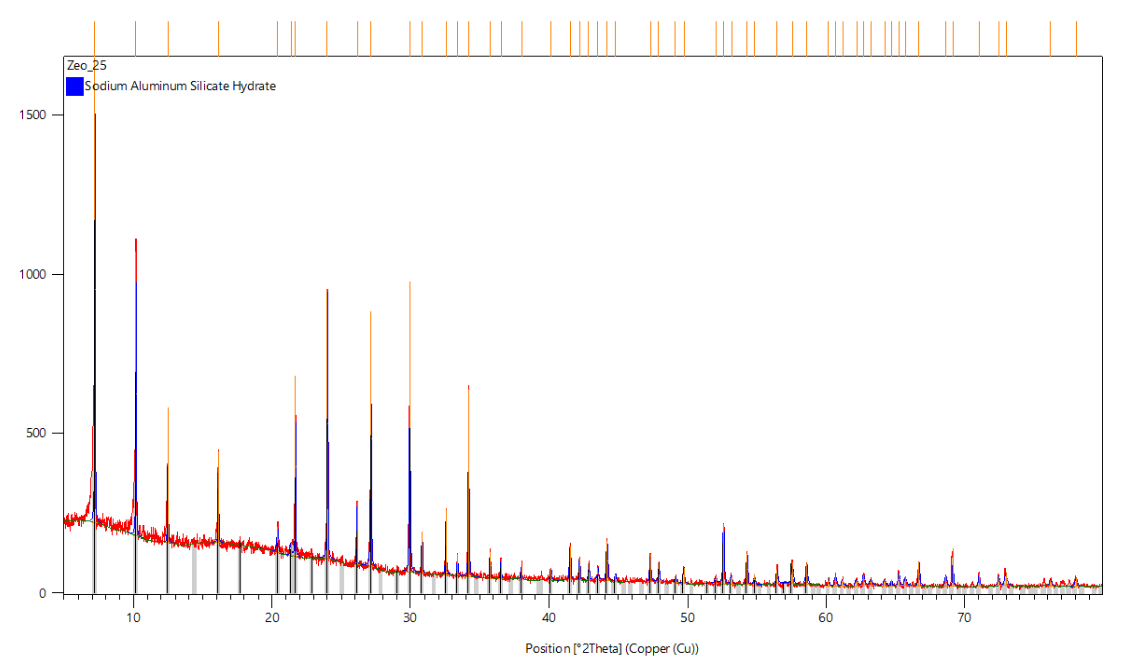
\includegraphics[scale=0.50]{Screenshot 2025-05-17 133057.png}
\end{center}
\caption{\textit{Zeigt das Pulverdiffraktogramm von hergestellten Zeolith A mit den Referenzreflexe mit dem Referenzcode 00-039-0222}}
\label{XRD}
\end{figure}
Anschließend wird mittels \mbox{HighScore-Plus} die Kristallstruktur untersucht. Dabei wurden die Einheitszelle untersucht.
Diese wurden mit den Theoretischen Werten des Referenzreflex verglichen dies wird in der Tabelle \ref{Kastenlänge} aufgezeigt.
\begin{table}[h!]
\caption{\textit{Zeigt die Theoretische und Festgestellte Einheitszelle von den hergestellten Zeolith As (Referenzcode 00-039-0222). Die Verfeinerung wurde mithilfe des Programmes HighScore Plus durchgeführt. }}
\begin{center}
\begin{tabular}{|>{\columncolor{lightgray}}>{\centering\arraybackslash}p{4cm}|>{\centering\arraybackslash}p{4cm}|>{\centering\arraybackslash}p{4cm}|}
   \hline
   \rowcolor{gray}
   &Theoretische& Festgestellte (Standardabweichung) \\
   \hline
   a[\AA]&\centering{24.6100}& 24.5847 (8)\\
   \hline
   b[\AA]&24.6100& 24.5847 (8)\\
   \hline
   c[\AA]&24.6100& 24.5847 (8)\\
   \hline
   $\alpha$[°]&90& 90\\
   \hline
   $\beta$[°]&90& 90\\
   \hline
   $\gamma$[°]&90& 90\\
   \hline
   Volumen[\AA$^3$]&14905.10 & 14859.21\\
   \hline

\end{tabular}
\label{Kastenlänge}
\end{center}
\end{table}



\subsection{Durchschnittliche Anzahl von Elementarzellen pro Kristall}
Zunächst wird die durchschnittliche Kristallgröße bestimmt. Dies erfolgt anhand von SEM-Aufnah-men. Dies ist in Abbildung \ref{SEm} dargestellt. Dabei handelt es sich nicht um Aufnahmen der selbst hergestellten Proben, sondern um bereitgestellte Vergleichsaufnahmen.

\begin{figure}[!h]
  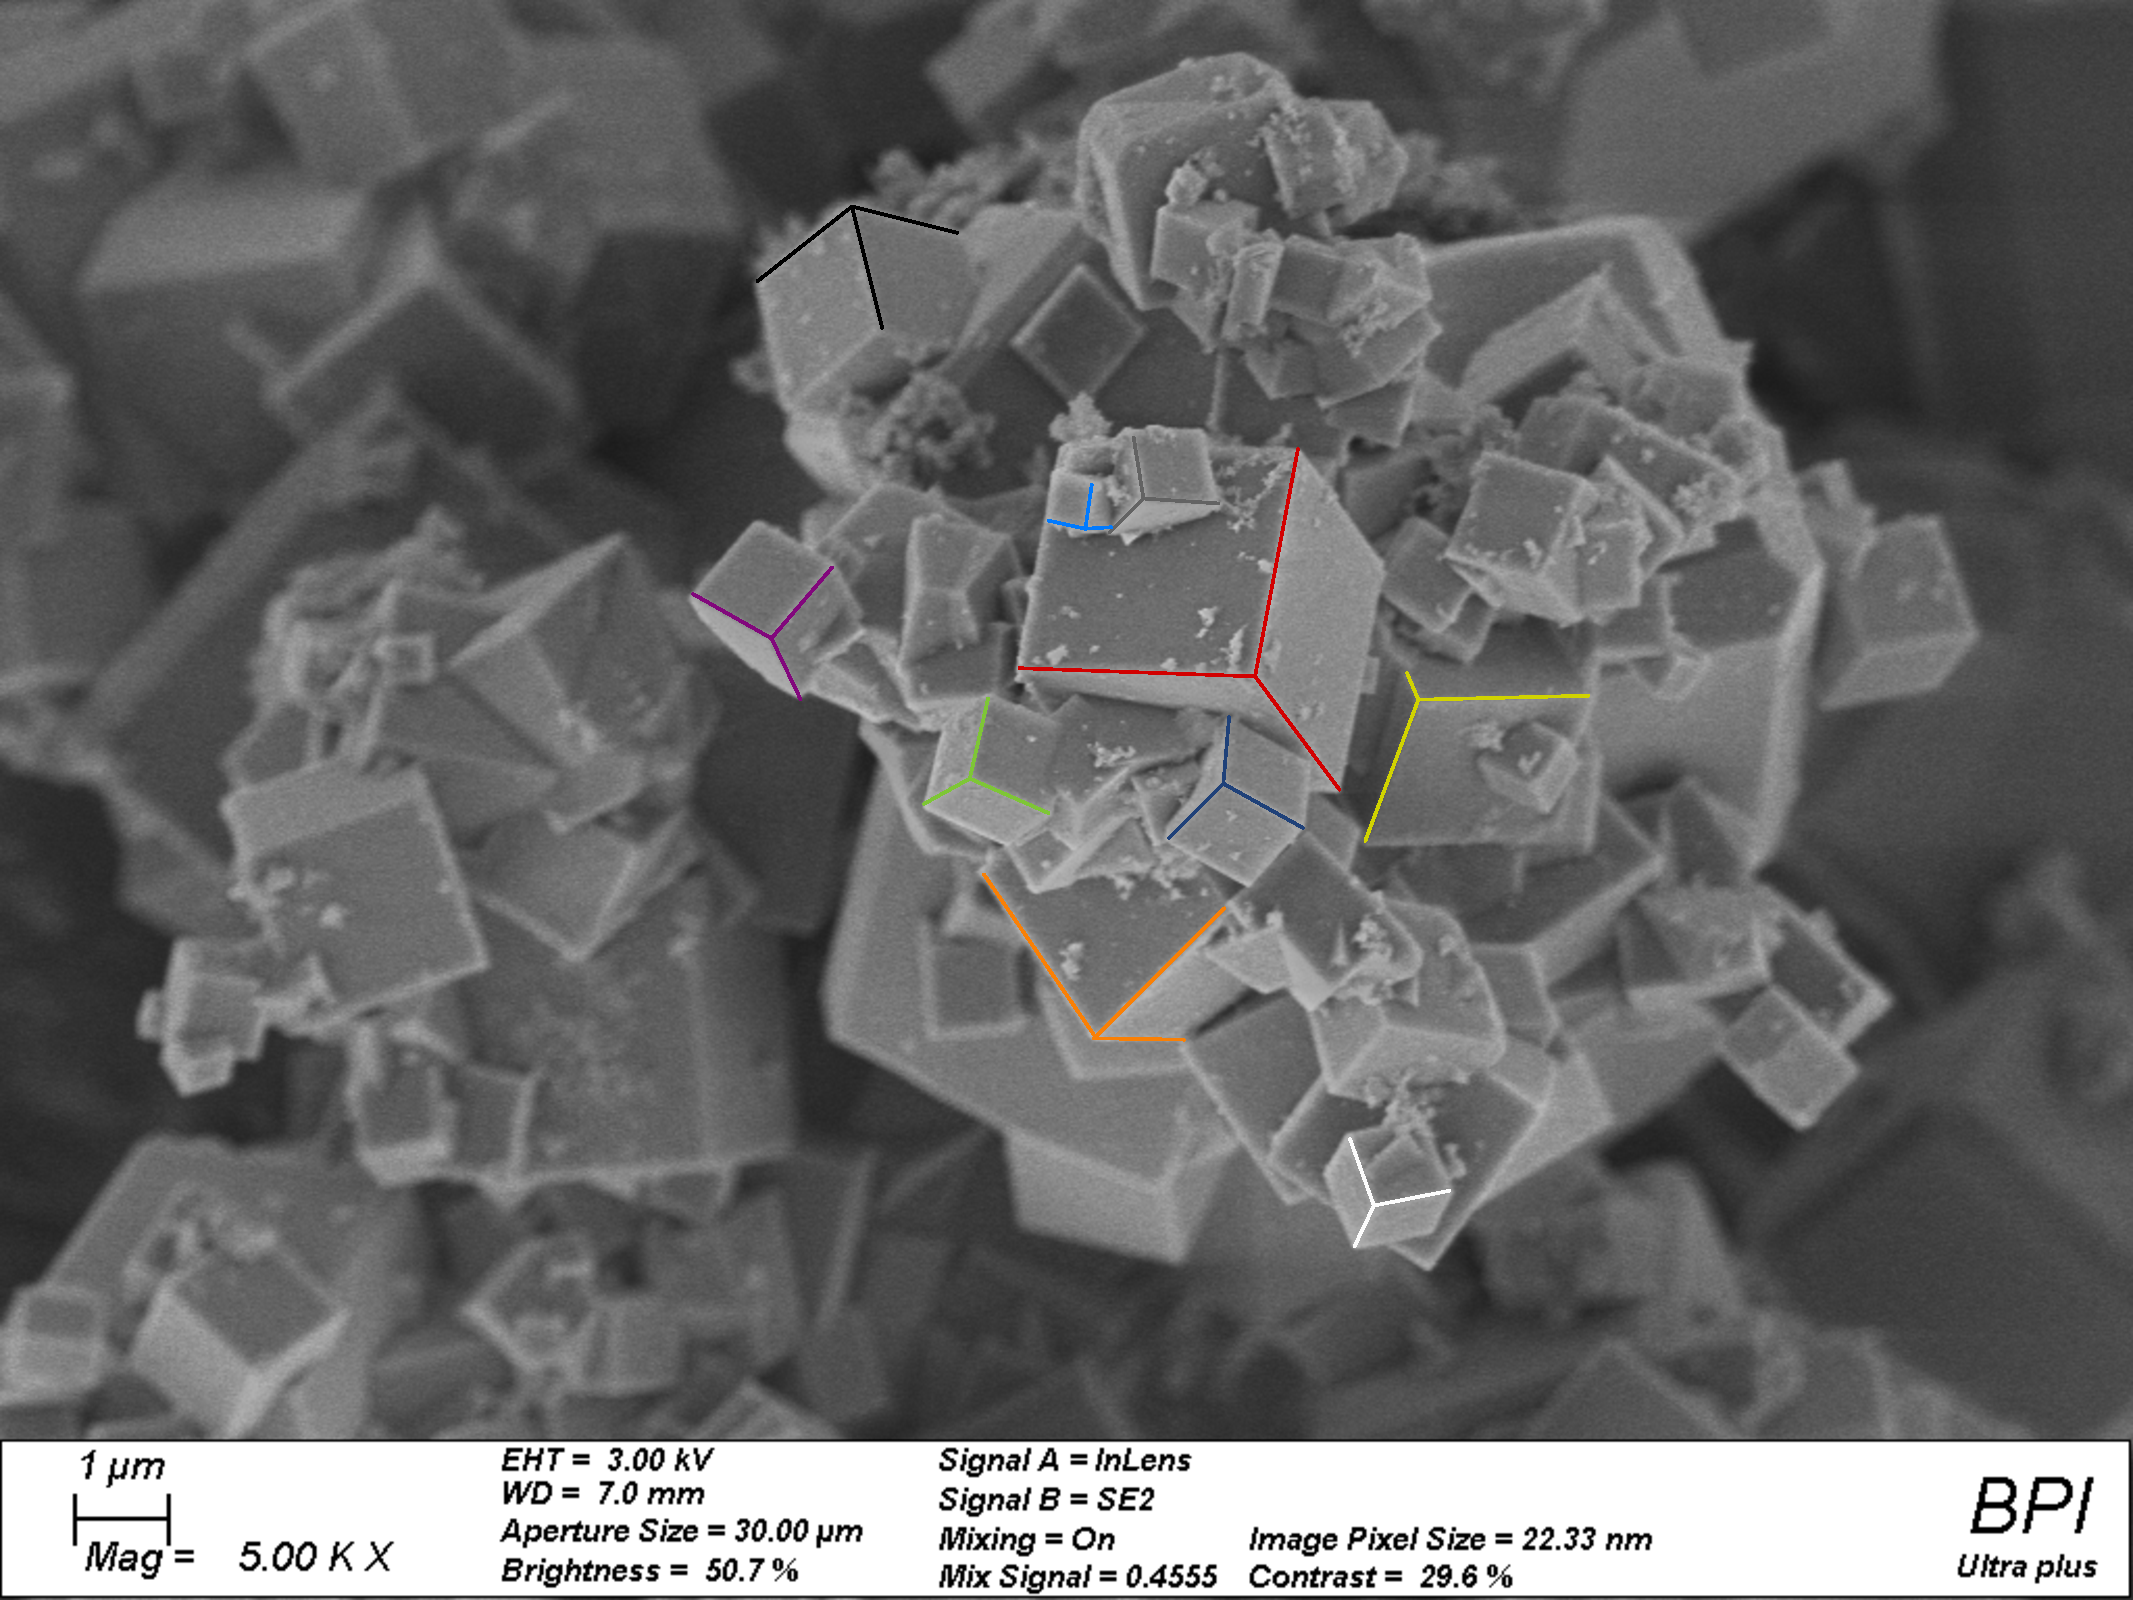
\includegraphics[width=\linewidth]{SEM_Zeo___25_.pdf}
  \caption{Zeigt die Sem-Aufnahme eines Zeolith, mit eingezeichneten Kristalle, deren Größe bestimmt werden soll.}
  \label{SEm}
\end{figure}

\noindent
Die Kristalle werden näherungsweise als Würfel angenommen. Aus der gemessenen Kantenlänge lässt sich das Kristallvolumen berechnen. Die Ergebnisse sind in Tabelle \ref{kristallgröße} dargestellt.
\newpage

\begin{table}[!h]
  \caption{zeigt die analysierten Kristalle mit den gemessenen Kantenlängen sowie den berechneten Volumina, wobei eine würfelförmige Geometrie angenommen wurde.}
  \label{kristallgröße}
\begin{tabular}{|>{\centering\arraybackslash}p{0.3\linewidth}|>{\centering\arraybackslash}p{0.3\linewidth}|>{\centering\arraybackslash}p{0.3\linewidth}|}
  \hline
  \rowcolor{gray}
  Marktierter Kristall aus der Abbildung \ref{SEm} & Kastenlänge [$\mu m$] & Volumen [$\mu m^3$]\\
  \hline
  Rot & 2.53& 16.19\\
  \hline
  Orange & 2.13 & 9.71 \\
  \hline
  Gelb & 1.80 & 5.83 \\
  \hline
  Schwarz & 1.33 & 2.37 \\
  \hline
  Lila & 1.00 & 1.00\\
 \hline
  Dunkelblau & 1.00 & 1.00\\
 \hline
  Grün & 1.00 & 1.00\\
\hline
Grau &0.80&0.51\\
\hline
Hellblau&0.40& 0.06\\
\hline
\end{tabular}

\end{table}

\noindent 
Aus Tabelle \ref{kristallgröße} wird die mittlere Kristallgröße bestimmt. Diese beträgt $\overline{V} = 4.19 \: \mu m^3$.
Daraus lässt sich die durchschnittliche Anzahl der Elementarzellen pro Kristallit bestimmen. Diese wird mithilfe der Formel \ref{durchschnittelementarzelle} berechnet.

\begin{equation}
  N_{Elemtarzellen} = \frac{V_{Kristall}}{V_{Elemtarzellen}} \cdot 8 = \frac{4.19 \: \mu m^3 }{1.485921 \cdot 10^{-6} \: \mu m^3} \cdot 8 =2.256 \cdot 10^{7}
  \label{durchschnittelementarzelle}
\end{equation}

\noindent
Daraus folgt, dass durchschnittlich $2.256 \cdot 10^7$ Elementarzellen pro Kristall vorliegen.






\subsection{\texorpdfstring{Austauschvermögen von Zeolith A der Kationen \ce{Ca^{2+}} und \ce{Na^{+}}}{Austauschvermögen von Zeolith A der Kationen Ca2+ und Na+}}
Die molare Masse MM von Zeolith A beträgt 17527.49 $\frac{g}{mol}$. Daraus lässt sich die Stoffmenge nn in einem Gramm Zeolith berechnen.
\begin{equation}
  n_{Zeolith}=\frac{m}{M}=\frac{1 g}{17527.49 \frac{g}{mol}}=5.71 \cdot 10^{-5} mol
  \label{stoffmenge}
\end{equation}

\noindent
Aus der in Gleichung \ref{stoffmenge} berechneten Stoffmenge lässt sich ermitteln, wie viele \ce{Ca^{2+}}-Kationen eingelagert werden können. Diese Anzahl entspricht der Hälfte der \ce{Na^+}-Kationen.
\begin{equation}
  n_{\ce{Ca^2+}}=\frac{1}{2} \cdot 96 \cdot n_{Zeolith}=2.741 \cdot 10^{-3} mol
  \label{Kalicium}
\end{equation}

\noindent
Die in Gleichung \ref{Kalicium} berechnete Stoffmenge wird nun in eine Masse umgerechnet, die 109,9 mg \ce{Ca^{2+}} entspricht. Theoretisch kann somit 1 g Zeolith 109,9 mg \ce{Ca^{2+}} aufnehmen.
Zur praktischen Überprüfung wird in 100 mL Leitungswasser zunächst auf \ce{Ca^{2+}} getestet. Anschließend wird 1 g Zeolith hinzugegeben und der Schnelltest erneut durchgeführt.
\newpage

\begin{figure}[ht]
    \centering
  \begin{subfigure}[b]{0.47\linewidth}
    \centering
    \includegraphics[width=\textwidth]{Wasserhärtelegende.png}
    \caption{Zeigt die Legende des Wasserhärteschnelltest}
    \label{ganz}
    
  \end{subfigure}
   \begin{subfigure}[b]{0.47\linewidth}
    \centering
    \includegraphics[width=\textwidth]{wasserhärtetests.png}
    \caption{Zeigt den Schnelltest vor der Zeolith Zugabe (oben) und danach (unten)}
    \label{zoom}
    
  \end{subfigure}
  \caption{Zeigt das Ergebnis des Wasserhärteschnelltest vor und nach der Zugabe von Zeolith A in Leitungswasser.}
  \label{Physisorption}
\end{figure}

\noindent
Aus Abbildung \ref{Physisorption} lässt sich ablesen, dass die Konzentration von \ce{CaCO3} vor der Zugabe des Zeoliths bei über 125 $\frac{mg}{L}$ lag. Nach der Zugabe von Zeolith A sank die Konzentration auf unter 55 $\frac{mg}{L}$. Daraus ergibt sich, dass mindestens 70 $\frac{mg}{L}$ \ce{CaCO3} entfernt wurden, was bei einem Probenvolumen von 100 mL einer absoluten Menge von 7 mg entspricht.

\noindent
Bei einer molaren Masse von \ce{CaCO3} von 100.01 g/mol entspricht dies einer Stoffmenge von \(6.999 \cdot 10^{-5}\) mol, also etwa 2.81 mg \ce{Ca^2+}. Dieser Wert liegt deutlich unter dem zuvor theoretisch berechneten Wert von 109.9 mg. Allerdings wurde bei dieser Berechnung mit der minimal möglichen Austauschmenge gerechnet, und es konnte nicht festgestellt werden, ob der Zeolith darüber hinaus noch mehr \ce{Ca^{2+}} hätte aufnehmen können.

\noindent
Da jedoch eindeutig \ce{Ca^{2+}}-Ionen ausgetauscht wurden, kann die Synthese des Zeolith As als erfolgreich angesehen werden.



\newpage
\section{Zusammenfassung}
In diesem Versuch wurde erfolgreich Zeolith A hergestellt. Anschließend wurde mithilfe einer SEM-Aufnahme bestimmt, dass durchschnittlich \(2.256 \cdot 10^7\) Elementarzellen pro Kristall vorliegen. Zudem sollte das Austauschvermögen des Zeoliths A gegenüber \ce{Ca^{2+}}- und \ce{Na^{+}}-Ionen untersucht werden. Dies war jedoch nicht vollständig möglich, da der Zeolith vermutlich mehr \ce{Ca^{2+}} aufnehmen kann, als im Leitungswasser vorhanden war.


\newpage
\section{Literaturverzeichnis}
\printbibliography







\end{document}